\begin{frame}
	\frametitle{Pong - Diagrama}
	
    \begin{center}
        Visión general del sistema
    \end{center}
	
    \begin{center}
		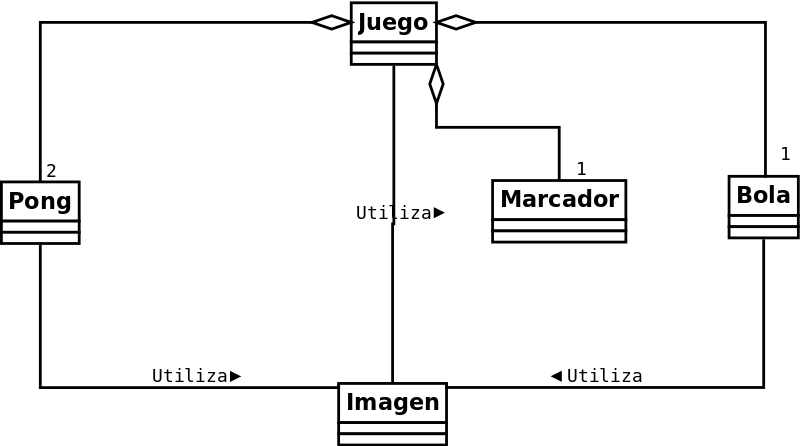
\includegraphics[scale=0.25]{img/modulos.png}
	\end{center}	

\end{frame}

\begin{frame}[fragile]
	\frametitle{Pong - Estructura del proyecto}
    
    \begin{columns}[c]
	\column{175pt}

\begin{verbatim}
|- pong
    |- makefile
    |- main.cpp
    |- motor
    |    |- fichero.c
    |    |- fichero.h
    |    |- (...)
    |
    |- multimedia
    |    |- imagen.png
    |    |- fuente.ttf
    |    |- (...)
\end{verbatim}
	
	\column{125pt}
	\begin{center}
		
\includegraphics[scale=0.4]{img/Binary-tree-256.png}
	\end{center}	
	
    \end{columns}

\end{frame}

\begin{frame}
	\frametitle{Pong - Paso 1}
	
	\begin{block}{Objetivos}
		\begin{itemize}
			\item Inicializar SDL
			\item Crear una ventana
			\item Esperar evento de salida
			\item Cerrar SDL
		\end{itemize}            
	\end{block}

\end{frame}

\begin{frame}[fragile]
    \frametitle{Pong - Paso 1 - SDL\_Init}
	
\begin{verbatim}
int SDL_Init(Uint32 flags);
\end{verbatim}

    \begin{block}{SDL\_Init}
	Inicia SDL y los subsistemas que queramos
	
	\emph{Parámetros}:
	\begin{itemize}
	    \item Uint32 flags: susbistemas a inicializar. Se combinan con $||$
		\begin{itemize}
		    \item SDL\_INIT\_TIMER
		    \item SDL\_INIT\_AUDIO
		    \item SDL\_INIT\_VIDEO
		    \item SDL\_INIT\_CDROM
		    \item SDL\_INIT\_JOYSTICK
		    \item SDL\_INIT\_EVERYTHING
		\end{itemize}
	\end{itemize}
	
	\emph{Devuelve}: $0$ si tiene éxito, $-1$ en caso contrario

    \end{block}

\end{frame}

\begin{frame}[fragile]
    \frametitle{Pong - Paso 1 - SDL\_Quit}
	
\begin{verbatim}
void SDL_Quit(void);
\end{verbatim}

    \begin{block}{SDL\_Quit}
	Cierra SDL y todos sus subsistemas
    \end{block}

\end{frame}

\begin{frame}[fragile]
    \frametitle{Pong - Paso 1 - atexit}
	
\begin{verbatim}
int atexit(void (*function) (void));
\end{verbatim}

    \begin{block}{atexit}
	Llama a una función de tipo \emph{void funcion(void)} al terminar la ejecución
	
	\emph{Parámetros}:
	\begin{itemize}
	    \item void (*function) (void): puntero a una función que recibe y devuelve void.
	    
	    Ejemplo:
	    \begin{verbatim}
	    atexit(SDL_Quit);
	    \end{verbatim}
	\end{itemize}
	
	\emph{Devuelve}: $0$ si tiene éxito, distinto si falla
    \end{block}

\end{frame}

\begin{frame}[fragile]
    \frametitle{Pong - Paso 1 - SDL\_SetVideoMode}
	
\begin{verbatim}
SDL_Surface *SDL_SetVideoMode(int width, int height,
                              int bpp, Uint32 flags);
\end{verbatim}

    \begin{block}{SDL\_SetVideoMode}
	Crea la superficie principal (nuestra ventana)
	
	\emph{Parámetros}:
	\begin{itemize}
	    \item int width: ancho en píxeles
	    \item int height: alto en píxeles
	    \item int bpp: bits por píxel (profundidad)
	    \item Uint32 flags: opciones:
	    \begin{itemize}
		    \item SDL\_HWSURFACE
		    \item SDL\_DOUBLEBUF
	    \end{itemize}
	\end{itemize}
	
	\emph{Devuelve}: superficie principal o NULL si hay erores
    \end{block}

\end{frame}

\begin{frame}[fragile]
    \frametitle{Pong - Paso 1 - SDL\_WM\_SetCaption}
	
\begin{verbatim}
void SDL_WM_SetCaption(const char *title,
                       const char *icon);
\end{verbatim}

    \begin{block}{SDL\_WM\_SetCaption}
	Establece título e icono de la ventana
	
	\emph{Parámetros}:
	\begin{itemize}
	    \item const char *title: cadena con el título ("Pong")
	    \item const char *icon: cadena con la ruta del icono
	\end{itemize}
    \end{block}

\end{frame}

\begin{frame}[fragile]
    \frametitle{Pong - Paso 1 - SDL\_ShowCursor}
	
\begin{verbatim}
int SDL_ShowCursor(int toggle);
\end{verbatim}

    \begin{block}{SDL\_ShowCursor}
	Muestra u oculta el cursor en la ventana
	
	\emph{Parámetros}:
	\begin{itemize}
	    \item int toggle: SDL\_ENABLE, SDL\_DISABLE o SDL\_QUERY (consultar)
	\end{itemize}
	
	\emph{Devuelve}: estado del cursor (SDL\_ENABLE o SDL\_DISABLE)
    \end{block}

\end{frame}

\begin{frame}[fragile]
    \frametitle{Pong - Paso 1 - TTF\_Init}
	
\begin{verbatim}
int TTF_Init();
\end{verbatim}

    \begin{block}{TTF\_Init}
	Inicializa librería auxiliar para fuentes
	
	\emph{Devuelve}: $0$ si tiene éxito, $-1$ en caso contrario
    \end{block}

\end{frame}

\begin{frame}[fragile]
    \frametitle{Pong - Paso 1 - SDL\_GetKeyState}
	
\begin{verbatim}
Uint8 *SDL_GetKeyState(int *numkeys);
\end{verbatim}

    \begin{block}{SDL\_GetKeyState}
	Captura el estado del teclado completo
	
	\emph{Parámetros}:
	\begin{itemize}
	    \item int *numkeys: aquí se almacena el número de teclas (podemos pasarle NULL)
	\end{itemize}
	
	\emph{Devuelve}: vector con el teclado mapeado.	Ejemplo:
\begin{verbatim}
teclado = SDL_GetKeyState(NULL);
if(teclado[SDLK_UP])
    /* Hemos pulsado arriba */
\end{verbatim}
\end{block}

\end{frame}

\begin{frame}
	\frametitle{Pong - Paso 1}
	
    \begin{center}
        \textbf{¡Hora de currar!}
    \end{center}
	
    \begin{center}
		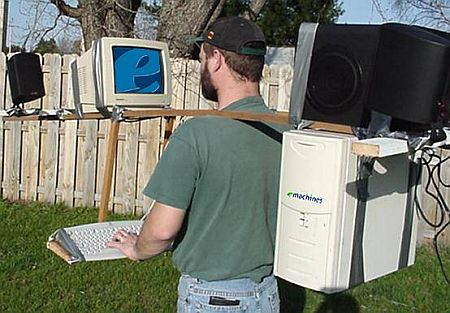
\includegraphics[scale=0.4]{img/currar-1.jpg}
    \end{center}	

\end{frame}

\begin{frame}
	\frametitle{Pong - Paso 1}
	
    \begin{center}
        \textbf{Resultado}
    \end{center}
	
    \begin{center}
		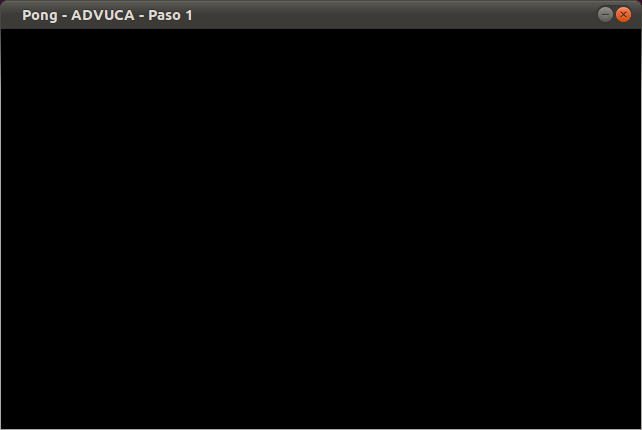
\includegraphics[scale=0.4]{img/pong-advuca-1.png}
    \end{center}	

\end{frame}

\begin{frame}
	\frametitle{Pong - Paso 2}
	
	\begin{block}{Objetivos}
		\begin{itemize}
			\item Módulo de carga y dibujado de imágenes
			\item Cargar mesa de juego
		\end{itemize}            
	\end{block}

\end{frame}

\begin{frame}[fragile]
    \frametitle{Pong - Paso 2 - IMG\_Load}
	
\begin{verbatim}
SDL_Surface *IMG_Load(const char *file);
\end{verbatim}

    \begin{block}{IMG\_Load}
	Carga una imagen
	
	\emph{Parámetros}:
	\begin{itemize}
	    \item const char *file: ruta de la imagen a cargar
	\end{itemize}
	
	\emph{Devuelve}: superficie con la imagen cargada, NULL si falla
    \end{block}

\end{frame}

\begin{frame}[fragile]
    \frametitle{Pong - Paso 2 - SDL\_DisplayFormatAlpha}
	
\begin{verbatim}
SDL_Surface *SDL_DisplayFormatAlpha(SDL_Surface *surface);
\end{verbatim}

    \begin{block}{SDL\_DisplayFormatAlpha}
	Adapta una superficie con transparencia al formato de la pantalla
	
	\emph{Parámetros}:
	\begin{itemize}
	    \item SDL\_Surface *surface: superficie a adaptar
	\end{itemize}
	
	\emph{Devuelve}: superficie con la imagen adaptada, NULL si falla
    \end{block}

\end{frame}

\begin{frame}[fragile]
    \frametitle{Pong - Paso 2 - SDL\_FreeSurface}
	
\begin{verbatim}
void SDL_FreeSurface(SDL_Surface *surface);
\end{verbatim}

    \begin{block}{SDL\_FreeSurface}
	Libera la memoria ocupada por la superficie
	
	\emph{Parámetros}:
	\begin{itemize}
	    \item SDL\_Surface *surface: superficie a eliminar
	\end{itemize}
    \end{block}
    
    \begin{center}
    \textbf{¡No se usa \emph{free(surface);} !}
    \end{center}

\end{frame}

\begin{frame}[fragile]
    \frametitle{Pong - Paso 2 - SDL\_BlitSurface}
	
\begin{verbatim}
int SDL_BlitSurface(SDL_Surface *src, SDL_Rect *srcrect,
                    SDL_Surface *dst, SDL_Rect *dstrect);
\end{verbatim}

    \begin{block}{SDL\_FreeSurface}
	Pega la superficie origen en la superficie destino
	
	\emph{Parámetros}:
	\begin{itemize}
	    \item SDL\_Surface *src: superficie origen
	    \item SDL\_Rect *srcrect: recuadro de la imagen origen a copiar
	    \item SDL\_Surface *dst: superficie destino
	    \item SDL\_Rect *drcrect: recuadro de la imagen destino a ocupar
	\end{itemize}
	
	\emph{Devuelve}: $0$ si todo va bien, $-1$ si falla.
    \end{block}

\end{frame}

\begin{frame}[fragile]
    \frametitle{Pong - Paso 2 - SDL\_Flip}
	
\begin{verbatim}
int SDL_Flip(SDL_Surface *screen);
\end{verbatim}

    \begin{block}{SDL\_Flip}
	Intercambia el buffer temporal con la ventana (muestra nuestro \emph{collage})
	
	\emph{Parámetros}:
	\begin{itemize}
	    \item SDL\_Surface *screen: superficie principal que representa a la ventana
	\end{itemize}
	
	\emph{Devuelve}: $0$ si todo va bien, $-1$ si falla.
    \end{block}

\end{frame}

\begin{frame}
	\frametitle{Pong - Paso 2}
	
    \begin{center}
        \textbf{¡Hora de currar!}
    \end{center}
	
    \begin{center}
		
\includegraphics[scale=0.4]{img/currar-2.jpg}
	\end{center}	

\end{frame}

\begin{frame}
	\frametitle{Pong - Paso 2}
	
    \begin{center}
        \textbf{Resultado}
    \end{center}
	
    \begin{center}
		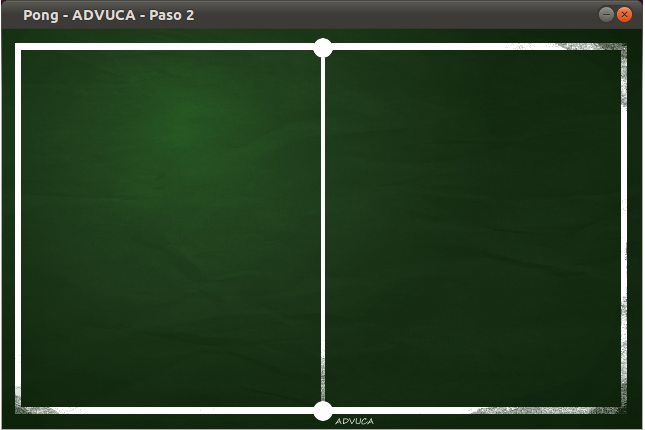
\includegraphics[scale=0.4]{img/pong-advuca-2.png}
	\end{center}	

\end{frame}

\begin{frame}
	\frametitle{Pong - Paso 3}
	
	\begin{block}{Objetivos}
		\begin{itemize}
			\item Módulo para las palas
			\item Control de la pala del jugador 1
			\item Control de FPS
		\end{itemize}            
	\end{block}

\end{frame}

\begin{frame}
	\frametitle{Pong - Paso 3}
	
    \begin{center}
        \textbf{¡Hora de currar!}
    \end{center}
	
    \begin{center}
		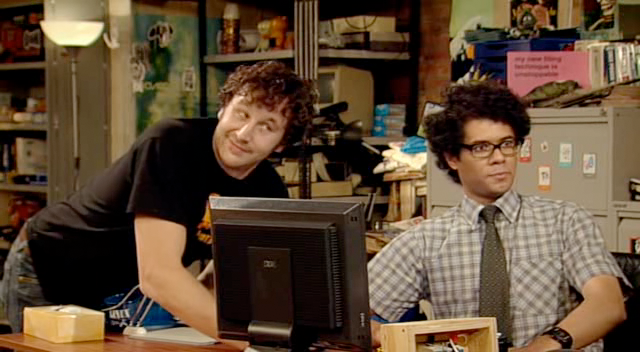
\includegraphics[scale=0.4]{img/currar-6.png}
	\end{center}	

\end{frame}

\begin{frame}
	\frametitle{Pong - Paso 3}
	
    \begin{center}
        \textbf{Resultado}
    \end{center}
	
    \begin{center}
		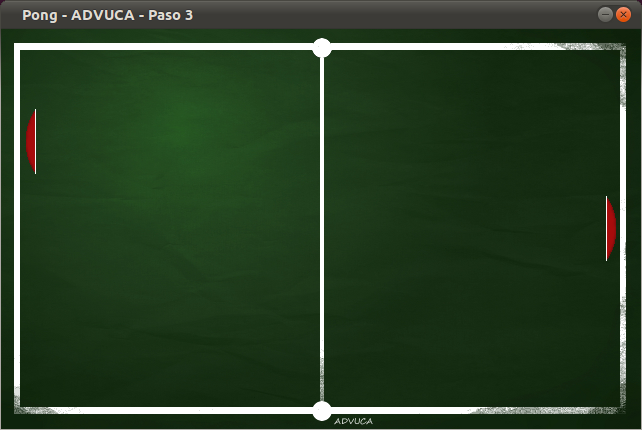
\includegraphics[scale=0.4]{img/pong-advuca-3.png}
	\end{center}	

\end{frame}

\begin{frame}
	\frametitle{Pong - Paso 4}
	
	\begin{block}{Objetivos}
		\begin{itemize}
			\item Módulo de la pelota
			\item Rebote básico de la pelota en bordes
			\item La pelota atraviesa las palas (por ahora)
		\end{itemize}            
	\end{block}

\end{frame}

\begin{frame}
	\frametitle{Pong - Paso 4}
	
    \begin{center}
        \textbf{¡Hora de currar!}
    \end{center}
	
    \begin{center}
		
\includegraphics[scale=0.4]{img/currar-4.jpg}
	\end{center}	

\end{frame}

\begin{frame}
	\frametitle{Pong - Paso 4}
	
    \begin{center}
        \textbf{Resultado}
    \end{center}
	
    \begin{center}
		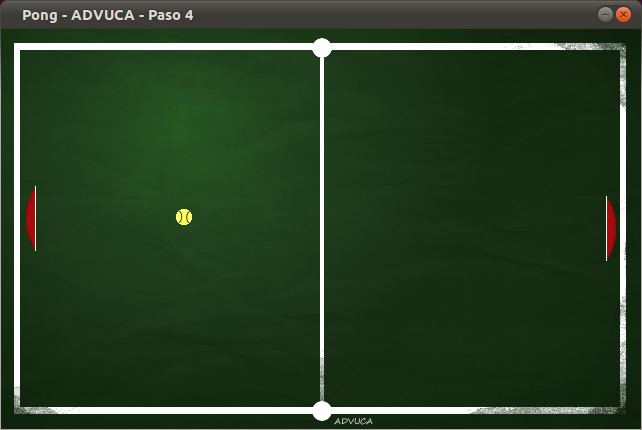
\includegraphics[scale=0.4]{img/pong-advuca-4.png}
	\end{center}	

\end{frame}

\begin{frame}
	\frametitle{Pong - Paso 5}
	
	\begin{block}{Objetivos}
		\begin{itemize}
			\item Colisión con las palas
			\item Inteligencia artificial
			\item La IA sigue a la pelota en el eje Y
		\end{itemize}            
	\end{block}

\end{frame}

\begin{frame}
	\frametitle{Pong - Paso 5}
	
    \begin{center}
        \textbf{¡Hora de currar!}
    \end{center}
	
    \begin{center}
		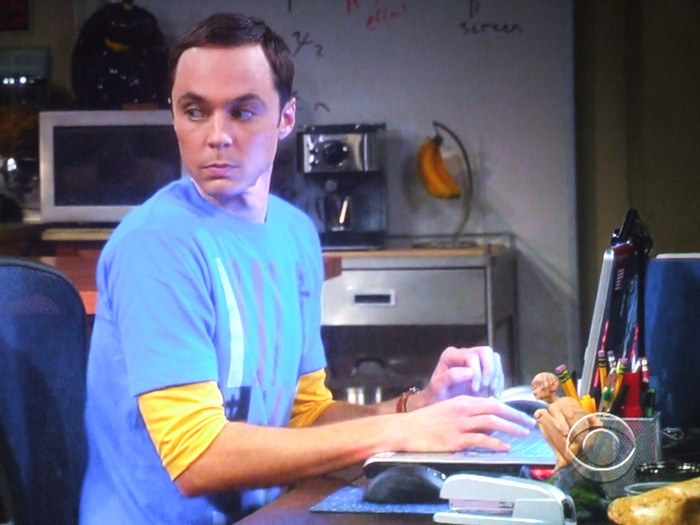
\includegraphics[scale=0.3]{img/currar-5.jpg}
	\end{center}	

\end{frame}

\begin{frame}
	\frametitle{Pong - Paso 5}
	
    \begin{center}
        \textbf{Resultado}
    \end{center}
	
    \begin{center}
		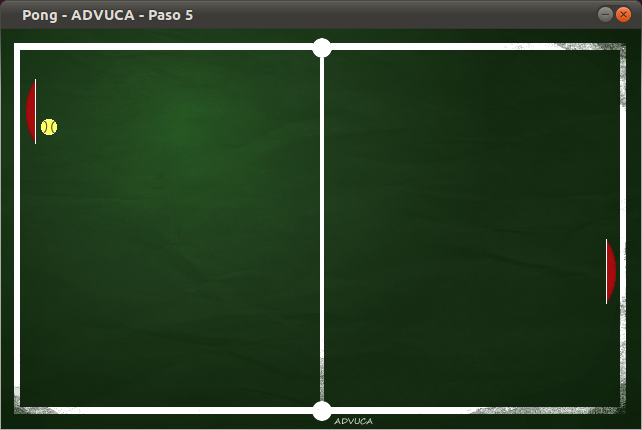
\includegraphics[scale=0.4]{img/pong-advuca-5.png}
	\end{center}	

\end{frame}

\begin{frame}
	\frametitle{Pong - Paso 6}
	
	\begin{block}{Objetivos}
		\begin{itemize}
			\item Creación del módulo marcador
			\item Si el jugador golpea la bola, suma un punto
			\item Se mantiene el récord de golpeos
			\item El marcador se reinicia si el jugador falla
		\end{itemize}            
	\end{block}

\end{frame}

\begin{frame}
	\frametitle{Pong - Paso 6}
	
    \begin{center}
        \textbf{¡Hora de currar!}
    \end{center}
	
    \begin{center}
		
\includegraphics[scale=0.7]{img/currar-3.jpg}
	\end{center}	

\end{frame}

\begin{frame}
	\frametitle{Pong - Paso 6}
	
    \begin{center}
        \textbf{Resultado}
    \end{center}
	
    \begin{center}
		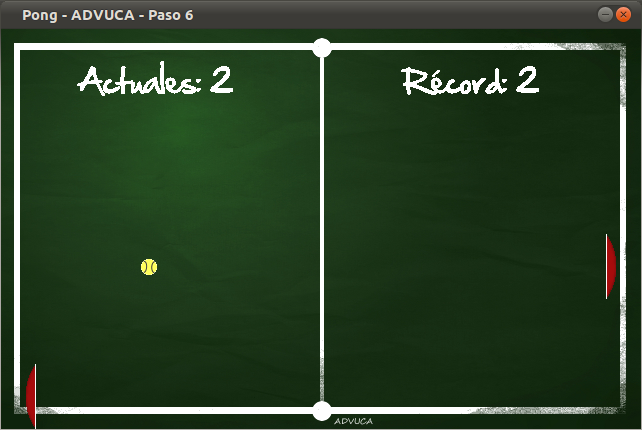
\includegraphics[scale=0.4]{img/pong-advuca-6.png}
	\end{center}	

\end{frame}
